\chapter{Methodology}

In this paper, I will meet the following challenges:
study properties and patterns of smart contracts and blockchains;
use neural networks to classify the source code of conventional applications;
transform conventional applications to smart contracts;
verify the correctness of smart contracts.


\section{Description of methods to solve the problem}

\paragraph*{Properties of Smart Contracts}
To tackle the first problem, I will perform literature review, find properties and patterns of smart contracts and blockchains people already discovered, and the tools they used.
For example, I learned the differences between smart contracts and {\dapp}~\cite{johnston2014general};
smart contracts are in the paradigm of duplicated computing~\cite{shae2018transform} instead of distributed computing;
\cite{yang2020implementation}~proposed a smart contract architecture model and used a finite-state machine to model the behavior.

Like~\cite{tolmach2021survey} mentioned, I am better off finding a (mathematical) model for smart contract which can help describe operations on blockchain. This model is usually described in graph theory, algebra, or communicating sequential processes (CSP).
As a result, I need to pick up theories of programming languages. I will investigate theoretical differences between smart contract and traditional local programs;
look into rCOS~\cite{ke2012rcos} which is a formal model-driven engineering method for component-based software;
define some partial order by refinement calculus to prove each conversion does not break pre- and post-conditions, etc.
I believe parallel properties and data persistence are two important aspects to look at.
To conclude this part of work, I will publish papers on the theory section of smart contracts.

\paragraph*{Identification of Functional Implementation}
I have already looked into using neural networks to analyze program source code.
As the first step, I innovatively classify commits into refactoring types, whether the commit is a variable renaming.
In the software engineering and neural network fields, few researchers explored commit classification and I got a paper published (see \autoref{sec:produced-publications}).
My paper used and expanded Jiang's dataset of 2 million commits collected from GitHub.
As soon as I learned the key characteristics a smart contract holds, I will train a neural network to automatically filter the conventional programs for the next transformation.


There are many neural architectures I can use, including the simplest dense layers, convolutional neural network~\cite{albawi2017understanding}, recurrent neural network~\cite{tarwani2017survey}, long short-term memory~\cite{skovajsova2017long}, to name but a few.

\begin{figure}[ht]
\centering
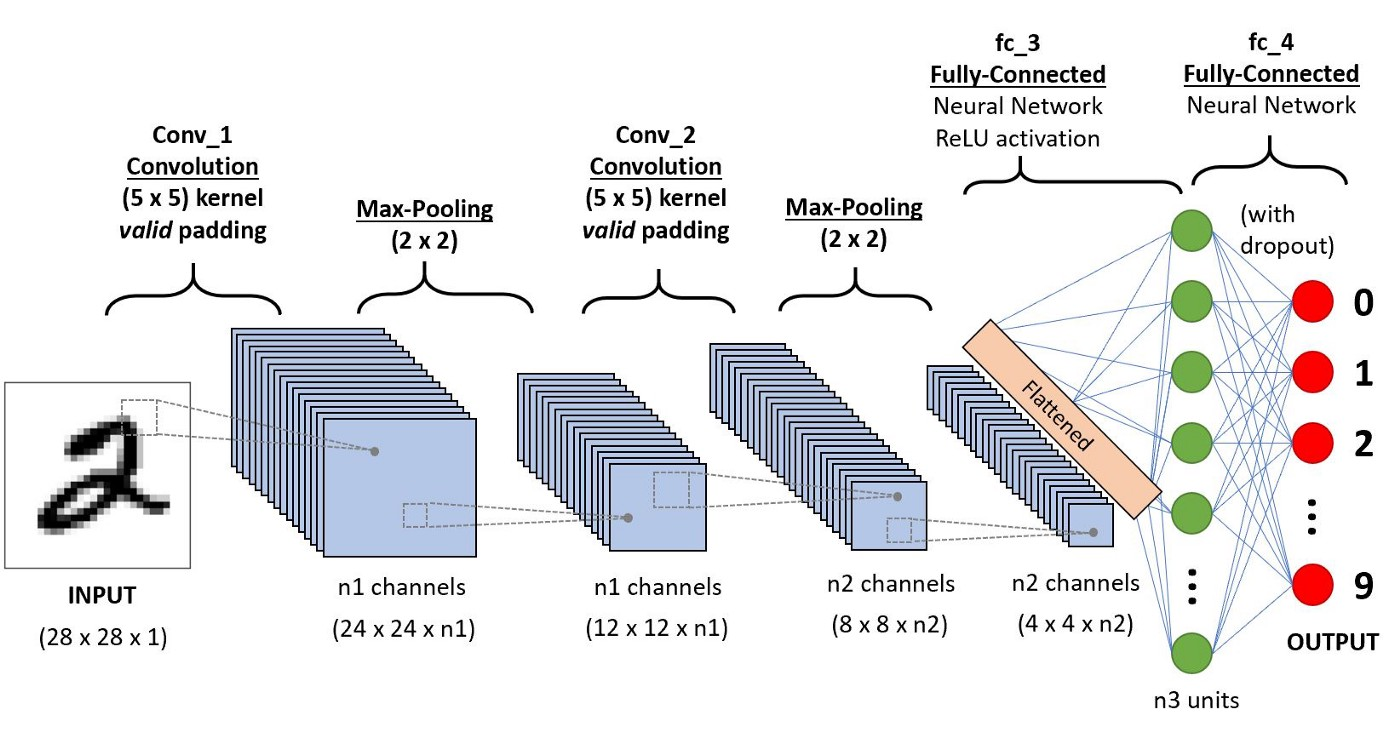
\includegraphics[width=0.9\linewidth]{cnn-big}
\caption{The architecture of CNN}
\label{fig:cnn}
\end{figure}

\autoref{fig:cnn}~is the architecture of convolutional neural network.
A Convolutional Neural Network (CNN) is a Deep Learning algorithm which can take in an input image, assign importance (learnable weights and biases) to various aspects/objects in the image and be able to differentiate one from the other. The pre-processing required in a CNN is much lower as compared to other classification algorithms. While in primitive methods filters are hand-engineered, with enough training, CNN has the ability to learn these filters/characteristics.
The architecture of a CNN is analogous to that of the connectivity pattern of Neurons in the Human Brain and was inspired by the organization of the Visual Cortex. Individual neurons respond to stimuli only in a restricted region of the visual field known as the Receptive Field. A collection of such fields overlap to cover the entire visual area.


\begin{figure}[ht]
\centering
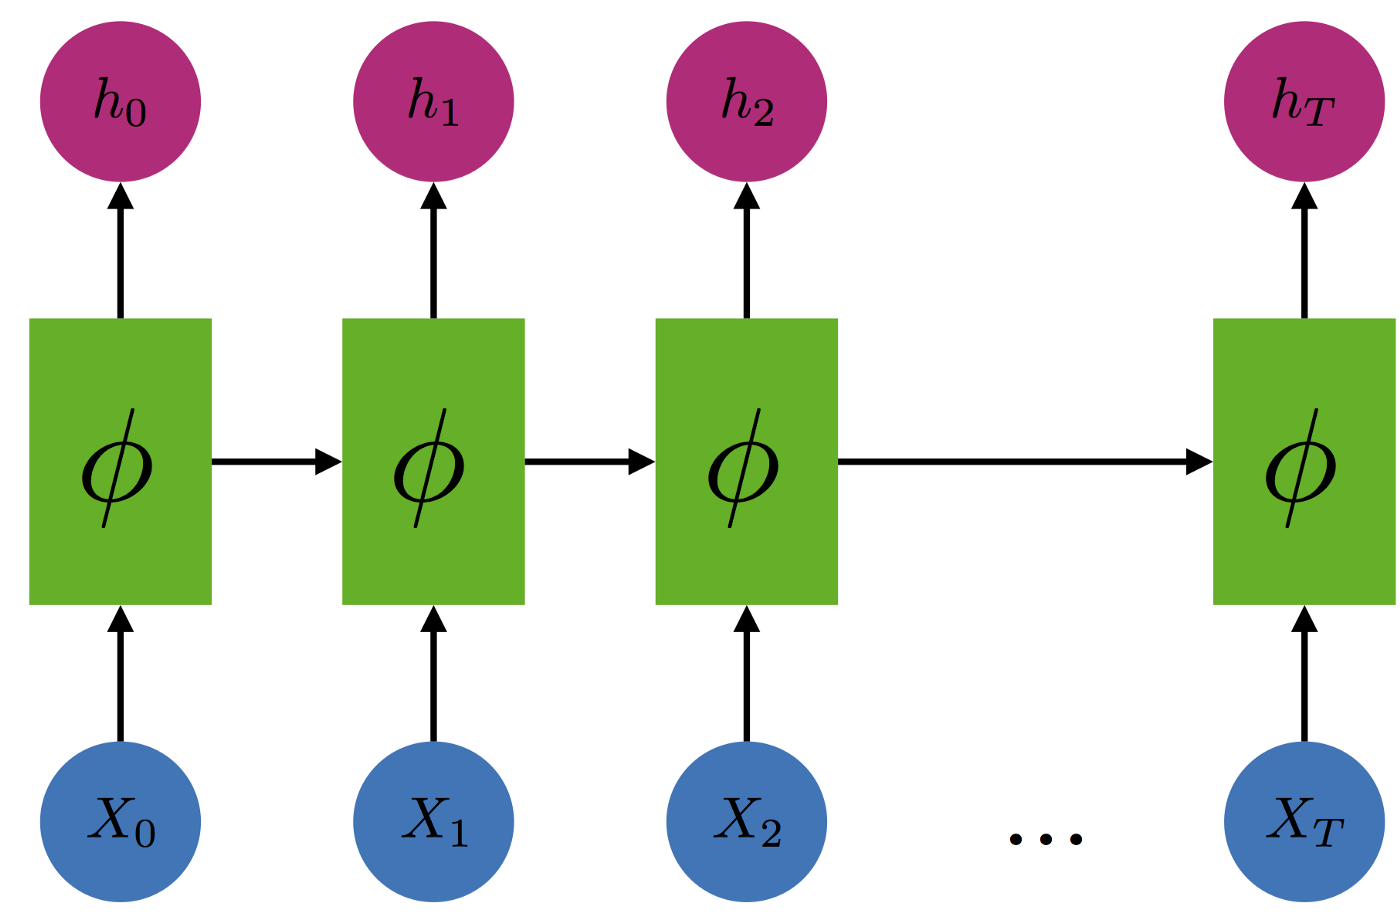
\includegraphics[width=0.7\linewidth]{rnn-big}
\caption{The architecture of RNN}
\label{fig:rnn}
\end{figure}

Recurrent neural network (RNN) consists of many blocks as seen in~\autoref{fig:rnn}.
The constituent block of RNN has two inputs $x_t$ and $x_{t-1}$, where  $x_t$ is the current time step input which can be a word of sentence, character of words, hertz of an audio etc. $x_{t-1}$ is previous time step input which is nothing but previous RNN block activation. Each input have their own weights, here we have two input with weights $Wx$ for $x_t$ and $Wa$ for $x_{t-1}$.
To calculate the loss of the model, individual block losses are calculated and summed up to get the total loss.

\begin{figure}[ht]
\centering
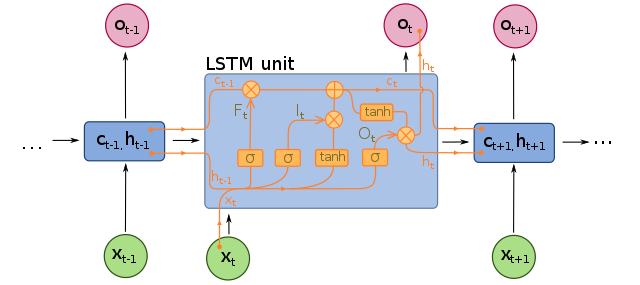
\includegraphics[width=0.7\linewidth]{lstm-big}
\caption{The constituent block of LSTM. The horizontal line is the flow of cell state.}
\label{fig:lstm}
\end{figure}

The architecture of Long Short-Term Memory (LSTM) is a specialized form of RNN. The constituent cell is depicted in~\autoref{fig:lstm}.
The key to LSTM is the cell state.
The cell state is like a conveyor belt. It runs straight down the entire chain, with only some minor linear interactions. It's very easy for information to just flow along it unchanged. LSTM has the ability to remove or add information to the cell state, carefully regulated by structures called gates.
LSTM has three different gates forget gate, input gate and output gate.


Given the numerous network architectures, I will first try the simplest dense layers on my neural network though I do not think the accuracy will be good.
CNN is for image processing so I will not use it.
I will focus more on RNN and LSTM.


In terms of the training dataset, I will take a similar approach and collect it from GitHub, probably with the help of the scraper~\cite{alexandru2017replicating}.
Categorical accuracy will be my evaluation metrics because my task is to classify source code.
I will also create confusion matrix in order to calculate false positive rate, accuracy, recall, f1-score, etc.


\paragraph*{Transformation to Smart Contracts}
Next, in order to transform functional implementation to smart contracts
I will base my work on RM2PT and develop a program called RM2Hyperledger, which generates executable source code in Java on Hyperledger Fabric platform.
Initially I will try rule-based transformation where the rules are hand-coded. Thereafter I will attempt on transformation by neural networks.

{\cocome} will be my first study case. I will make sure it can be correctly transformed to a blockchain smart contract. Then I will evaluate my algorithm on other study cases, e.g., SLEX-Web and ECefblock.


Data persistence of smart contract is a challenge.
The API of the blockchain platform is pretty general and naive. It treats the blockchain as a key-value store and there is no relation in objects. One object must hold an unique identifier (PK) of another object, and load the object from the chain when needed through the PK.
At present, most blockchain systems store data on-chain, i.e., the system saves application data to the chain, and then loads the data from the chain for execution.
Another off-chain method refers to storing the hash value of the data on the chain, and using the hash value as an index, storing the complete contract code on a different source.
For my project, I will pilot the on-chain approach due to its simplicity. I will add or locate PK of each entity, and add serialization support.

Another potential contribution in this area is to invent a library for saving and loading data to blockchain like Object Relational Mapping because
not all applications care the exact details of synchronizing object changes happening in memory to the blockchain.

When a method of a smart contract is called, the results are not yet committed to the chain until miners verified the results and reached a consensus. Hence, the post-condition checking may not happen within the smart contract. I will evaluate multiple way in implementing the post-condition, including a second smart contract, checking program local states, custom consensus algorithm, and lazy evaluation.
I shall also check blockchain validation frameworks and review how other blockchain programs were implemented.

After my conversion tool is implemented, I hope to let people try it so that I can find out how much my tool can actually save people's time given even experienced developers find it's hard to code smart contracts correctly~\cite{dao2019challenges}, and see to what extend people have to revise the auto-generated code. Then I will list these numbers in my paper for practically proving the effectiveness of my tool.



\paragraph*{Verification of Smart Contracts}
The input document of RM2PT uses OCL to describe invariants, pre- and post-conditions of an operation, and RM2PT transforms them to Java expressions.
My RM2Hyperledger should do that same but as~\cite{li2020securing} stated, adding these checks to all operations causes a huge runtime overhead because these checks read data from blochchain, which is a costly operation.
Nevertheless, I can utilize the results found in the earlier phase and perform static analysis.
After I got a formal mathematical model, I can use the model to prove the smart contract does not go into a bad state or the coin won't be stolen.
A SMT solver will be used.
But as smart contracts frequently interact with unverified, potentially adversarial outside code,
the assumptions that people can soundly prove are quite limited~\cite{bram2021rich}.

Inserting assertions into the implementation is runtime verification, which is still powerful though.
By checking locks and other invariants, we can make sure e.g., inter-smart contract reentrancy does not corrupt the memory.


%When a prototype is generated by my tool, it is still far from being a product, as the state-of-the-art code generation systems leave holes where the system is uncertain or the operation involves  third-party API or sorting. In addition, the prototype must be refactored and improved to meet non-functional requirements, e.g., aesthetic guidelines on the GUI.
%
%In the further coding, developers make commits which improves the system bit by bit, and each commit is essentially a diff. To process diff, neural network is again a key. I expect to use text vectorization layers to split the diff text into words, and use word embeddings to convert each word into a vector of decimals.
%
%
%A similar evaluation is desired to measure the effectiveness of the commit analysis tool. I may divide participants into two groups, one group uses the tool and the other does not use. I will compare how much productivity increase the group using the tool has comparing to the other group.
%

